\chapter{数值模型的建立和验证}
数值模拟已经成为内燃机设计开发和优化过程中的一个重要研究手段。由于内燃机工作过程中缸内形成高温和高压的环境
现有的测试方法很难直接将传感器安装在缸内进行测量,因此数值模拟在内燃机工作过程的研究上得到了广泛应用。
\section{离子电流模型}
点燃式发动机缸内混合气在火花点火、火核形成、火焰传播等燃烧过程中会产生大量的自由电子、正负离子和自由基等带电粒子,使燃气具有
一定的电导性。如果在火花塞两级施加一个稳定的直偏电压,由于有外加电场存在,带电粒子发生定向迁移,从而形成了火花塞离子电流。\par
以下的离子电流模型是基于以下的几个假设而成立的:
\begin{itemize}
\item 火花塞间隙中的燃气完全燃烧
\item 燃烧过程满足绝热过程
\item 燃气满足热力学平衡
\item 火花塞间隙近似成圆柱模型
\end{itemize}
\subsection{缸内燃烧化学反应式}
离子电流根据火焰的传播过程主要分为火焰前锋期和火焰后期。点火开始后,火焰前锋面从火花塞点火处开始燃烧,此时形成离子电流的火焰
前锋期;当火焰前锋面离开火花塞两端时为离子电流的火焰后期。其中火焰前锋期的主要化学反应如下:
\begin{align}
CH+O\stackrel{K_{1}}{\longrightarrow}CHO^{+}+e^{-}\\
CHO^{+}+H_{2}O\stackrel{K_{2}}{\longrightarrow}H_{3}O^{+}+CO\\
CH+C_{2}H_{2}\stackrel{}{\longrightarrow}C_{3}H_{3}+e^{-}\\
H_{3}O^{+}+e^{-}\stackrel{K_{3}}{\longrightarrow}H_{2}O+H
\end{align}
其中$K_{i}(i=1,2,3)$表示反应常数,大小分别为:
\begin{align}
K_{1}=5\times10^{-14}cm^{3}/s\\
K_{2}=7\times10^{-9}cm^{3}/s\\
K_{3}=2.3\times10^{-9}cm^{3}/s
\end{align}
由式可以看出,$K_{2}$大于$K_{1}$,也就是说火焰前锋中的离子大部分转化为$H_{3}O^{+}$,$K_{3}$
虽然也较大,但是由于反应不剧烈,因此在后火焰区$H_{3}O^{+}$还会存在。\par 
在后火焰期,导致$H_{3}O^{+}$的快速放热反应基本完成,$H_{3}O^{+}$基本上消失。此时的燃气温度可能在$1500^{\circ}C$以上,高温下的热电离决定了离子电流的变化。
焰后区内产生电离过程的主要物质是一氧化氮,研究表明\cite{reinmann1997local},95\%的有效的自由电子是由于$NO$的热电离产生的。
$NO$起主导作用的原因见表\ref{tab:nozx},$NO$的电离能在燃气内主要物质中是最小的,
\begin{table}[!h]
	\centering
	\caption{燃气中主要物质的电离参数}
	\label{tab:nozx}
	\begin{tabular}{c|rl|c|c}
		\toprule[1.5pt]
		物质			    &    \multicolumn{2}{c|}{电离能$/eV$}    &    浓度(在$15^{\circ} CA\ ATDC$时)    &    电离率\\\midrule[1pt]
		$NO$    		&   9.264&05     	&$1.48 \times 10^{-2}$  &  $2.44 \times 10^{-8}$\\
		$H_{2}O_{2}$    &   10.540&00 		&$1.60 \times 10^{-6}$  & $1.73 \times 10^{-9}$\\
		$CO$			&	14.013&90		&$4.85 \times 10^{-2}$	& $1.30 \times 10^{-12}$\\
		$CO_{2}$		&	13.777&00		&$7.17 \times 10^{-2}$	& $2.10 \times 10^{-12}$\\
		$H_{2}O$		&	12.618&80		&$1.16 \times 10^{-1}$	& $2.33 \times 10^{-11}$\\
		$N_{2}$			&	15.580&80		&$6.99 \times 10^{-1}$	& $5.03 \times 10^{-14}$\\
		$H_{2}$			&	15.425&89		&$9.72 \times 10^{-3}$	& $6.87 \times 10^{-14}$\\\bottomrule[1.5pt]
	\end{tabular}
\end{table}
这样,$NO$的电离率比其他物质的要大很多。大部分$NO$在$1000^{\circ}C$以上的温度根据Thermal或
Zeldovich\cite{zeldovich1946oxidation}机理形成,其后火焰期的主要化学反应为:
\begin{align}
O+N_{2}\longleftrightarrow NO+N\\
N+O_{2}\longleftrightarrow NO+O\\
N+OH\longleftrightarrow NO+H
\end{align}
\par
由于在高温高压的环境下$NO^{+}$浓度增加;当压力最大时,$NO^{+}$浓度达到最大,而对应的离子电流也达到峰值。
所以火焰后期的离子电流和缸内压力有很明确的关系。\par
总的来说,火焰前锋期的离子电流主要是化学电离产生的$H_{3}O^{+}$导致的;火焰后期的离子电流主要是$NO$热电离产生的电子导致的。
\subsection{离子电流产生的基本原理}
当火花塞两级加上偏置电压$U$时,火花塞间隙内会形成一个电场,如果此间燃气为等离子体状态,即存在带电粒子,那么这些带电粒子
的运动为自身的无规则热运动和电场方向迁移运动的叠加。如果他们在$dt$时间内分别移动了$dx_{i}$和$dy_{i}$距离,并使电极
上产生的面电荷密度的变化量为$q_{i}$和$q_{e}$,既有
\begin{equation}
q=q_{i}+q_{e}=en_{i}dx_{i}+en_{e}dx_{e}
\end{equation}
式中:$n_{i}$、$n_{e}$是正负带电粒子的浓度;$e$为元电荷的电量即一个电子所带的电荷。那么,在离阴极$x$距离处的电流密度为
\begin{equation}
j_{e}(x)=\frac{aq}{dt}=en_{i}v_{di}+en_{e}v_{de}
\end{equation}
式中$v_{di}$、$v_{de}$为正负带电粒子的迁移速度。\par 
对外电路而言,形成的火花塞离子电流为
\begin{equation}
I_{on}=\int_{A} j_{e}dA=j_{e}\pi r^{2}=(en_{i}v_{di}+en_{e}v_{de})\pi r^{2}
\end{equation}
式中$r$为火花塞中心电极的半径。
\subsection{带电粒子迁移速度的数学表达}
\subsubsection*{离子的迁移率$\mu_{i}$}
Langevin根据气体动力学,分析推导出离子的迁移率为
\begin{equation}
\mu_{i}=0.815\frac{e\overline{\lambda}}{M\ddot{v}}(\frac{M+M_{a}}{M})^{\frac{1}{2}}
\end{equation}
式中:$M$和$M_{a}$分别为离子和气体原子的质量;$\ddot{v}$为离子的均方根速度;$\overline{\lambda}$为离子在气体中的平均自由程。\par 
从上式可以看,$\mu_{i}$与电场强度$E$无关,这是由于上式推导是在$E/p$比较低的情况下进行的。实际上当$E/p$增大时,
$\mu_{i}$将于电场强度$E$有关。可以用一个经验公式表达,即
\begin{equation}
\mu_{i}=\mu_{0}[1+\alpha(\frac{E}{p})]^{\frac{1}{2}}
\end{equation}
式中:$\mu_{0}$为单位压强下离子的迁移率;$\alpha$为迁移常数,数值由实验测得;$E$为电场强度;$p$为气体压强。
\subsubsection*{电子的迁移率$\mu_{e}$}
电子和离子的迁移运动由于本身的特性差异很大,如下表\ref{tab:lzdz}所示。所以在处理电子迁移运动时,不能完全按照离子迁移运动的方式来
处理,经过公式推导,可以得到电子的迁移率为:
\begin{equation}
\mu_{e}=\frac{1}{3}e\overline{\lambda}(\frac{2}{\kappa Tm})^{1/2}
\end{equation}
\par  在燃气等离子体中,带电粒子在电场作用下会产生扩散和迁移运动;其根本原因是它们之间交换着能量和变更着位置。带电粒子的扩散和迁移反映出火花塞
离子电流的基本特性。
\begin{table}[!h]
	\centering
	\caption{离子和电子的比较}
	\label{tab:lzdz}
	\begin{tabular}{c|c|c}
	\toprule[1.5pt]
	&电子&离子\\
	\midrule[1pt]
	质量&小&大\\
	平均热运动& 大&小\\
	能量积累&可以&不可以\\
	碰撞面积&小&大\\
	刚体碰撞&否&是\\
	\bottomrule[1.5pt]
	\end{tabular}
\end{table}
\subsection{火花塞离子电流的数学模型}
\subsubsection*{火焰前期离子电流模型}
根据火焰前锋期的化学反应方程式可以得到各反应物和生成物的生成率。下式是$H_{3}O^{+}$在反应过程中满足的公式
\begin{equation}
\frac{d[H_{3}O^{+}]}{dt}=k_{2}[CHO^{+}][H_{2}O]-k_{3}[H_{3}O^{+}][e]
\end{equation}
当上式右边为零时,即为燃起的化学反应达到了平衡状态。同理,其他的反应物和生成物也满足类似的公式。于是可以得到:
\begin{equation}
%	[H_{3}O^{+}]=\frac{k_{2}[CHO^{+}][H_{2}O]}{k_{3}[e]}\\
%	[CHO^{+}]=\frac{k_{1}[CH][O]}{k_{2}[H_{2}O]}
	[H_{3}O^{+}]=[e]=(\frac{k_{1}[CH][O]}{k_{3}})^{1/2}
\end{equation}
\par  $[CH]$和$[O]$的平衡浓度主要取决于被点燃燃油混合气的空燃比。Reinman等人\cite{reinmann1997local}的研究表明,在空燃比$\phi_{at}$大于0.8的稀混合气条件下,$[H_{3}O^{+}]$可表示为
\begin{equation}
	[H_{3}O^{+}]=\frac{c}{\sqrt{\phi_{at}}}
\end{equation}
式中$c$为常数。\par 
现在已经求得了离子浓度,火花塞离子电流可以得到为
\begin{equation}
	I_{on}=en_{e}\pi r^{2}E\mu
\end{equation}
式中:$n_{e}$为相应于离子浓度的自由电子浓度;$v_{d}$为迁移速度;$E$为电厂强度;$\mu$为迁移速率;$e$为单位电荷。这里将反应区看成一个简单的
圆柱体,所以截面半径为$r$。
\subsubsection*{火焰后期的离子电流模型}
火焰后期离子电流主要收到$NO$的热电离的影响,而不是化学电离。首先计算出燃烧产物中的$NO$的浓度,然后可利用沙哈(Saha)方程求解$NO$在特定条件下发生热电离生成$NO^{+}$和
自由电子的电离率,并结合自由电子和离子的在外加电场作用下的迁移速率,就可以推导出火焰后期火花塞离子电流的数学模型。\par 
沙哈方程的公式如下:
	\begin{equation}
		\frac{\chi^{2}}{1-\chi^{2}}p=\frac{(2\pi m_{e})^{3/2}}{h^{3}}(\kappa T)^{5/2}exp(-\frac{E_{i}}{\kappa T})
	\end{equation}
其中:$m_{e}$为电子质量;$h$为普朗克质量;$\kappa$为波尔兹曼常数;$T$为气体的绝对温度;$E_{i}$为电离能;$p$为缸内压力;$\chi$为电离率。\par 
如果将火花塞间隙局部看成一个圆柱形的等离子体,那么有
\begin{equation}
	I_{on}=eN_{a}\chi \mu E\pi r^{2}
\end{equation}
其中$N_{a}$为离子浓度。
离子浓度满足公式
\begin{equation}
	\frac{dN_{a}}{dt}=6\times10^{16}T_{eq}^{-1/2}exp[-\frac{69090}{T_{eq}}](O_{2})_{eq}^{1/2}(N_{2})_{eq}
\end{equation}
于是可以得到火花塞离子电流公式为
\begin{equation}
	I_{on}=e^{3/2}N_{a}\pi r^{2}(\frac{\kappa}{2})^{1/4}\sqrt{\frac{3.2\times10^{-2}}{pm_{e}\overline{\lambda}}ET^{5/2}exp(-\frac{E_{i}}{\kappa T})}
\end{equation}
其中$p$为缸内压力;$E$为外加电场强度;$r$为火花塞中心电极半径;$\overline{\lambda}$为电子平均自由程;$T$为气体的绝对温度;$E_{i}$为电离能;$m_{e}$为电子质量;
$\kappa$为波尔兹曼常数。
\section{电路结构的简化模型}
\subsection{电容式离子电流电路结构}
如下图\ref{fig:ionstruct}所示的是电容式离子电流检测电路结构
\begin{figure}[!h]
	\centering
	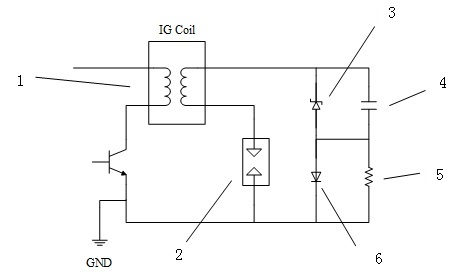
\includegraphics{thesis_figure/ion_struct}
	\caption{电容式离子电流检测电路结构}
	\label{fig:ionstruct}
\end{figure}
\par $1$表示点火线圈
\par $2$表示火花塞电极两段
\par $3$表示瞬态抑制二极管,防止电压过高使电路失效
\par $4$是电容,作为次级电路电源
\par $5$是检测电阻
\par $6$是普通二极管,用于限定检测电阻两端最大电压
\subsection{电容式离子电流曲线}
电容式离子电流分为三个时期:点火干扰期,火焰前锋期和火焰后期。如下图\ref{fig:ion_basic}所示是离子电流的三个时期。
\begin{figure}[!h]
	\centering
	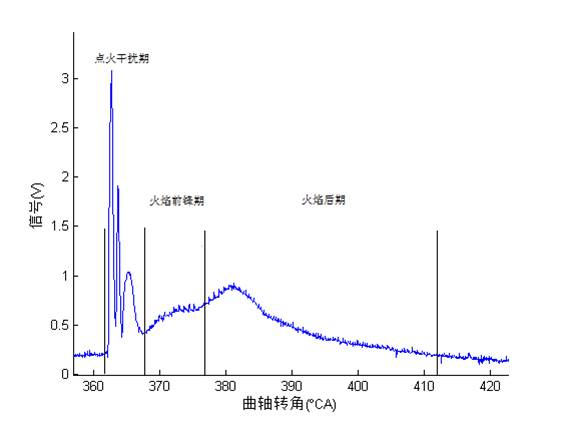
\includegraphics[width = 0.8\textwidth]{thesis_figure/model_chapter/ion_basic}
	\caption{电容式离子电流的三个时期}
	\label{fig:ion_basic}
\end{figure}
其中点火干扰期是由点火干扰造成的。火焰前锋期由火焰锋面经过电极附近的化学电离导致的;火焰后期由火焰锋面离开电极附近后的$NO$的热电离导致的。由于点火干扰的持续时间
和点火线圈的内部结构有关系,而火焰前锋期和火焰后期和燃烧有关系,所以点火干扰期可能会和火焰前锋期甚至是火焰后期相重合。但是点火干扰的曲线和火焰前锋或火焰后期的区别在于,点火干扰
期的曲线存在稳定的震荡信号,而化学电离或热电离导致的电流频率较低。通常来说火焰后期持续到整个燃烧阶段结束。
\subsection{火花塞动态电路模型}
火花塞结构复杂,但针对电磁干扰问题,主要考虑点火过程的放电通路,因此对其作适当的简化后的结果如图\ref{fig:hhsstruct}所示,其中金属外壳接地,具有耐高温、耐高压的氧化铝陶
瓷作为绝缘体,内置电阻由导电碳粉制成,中心电极为镍铜合金\cite{zyl2011}。
\begin{figure}[!h]
\centering
	\begin{minipage}[b]{0.5\textwidth}
		%\centering
		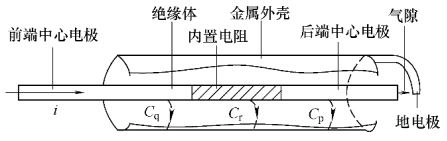
\includegraphics[width=\textwidth]{thesis_figure/anecdote_struct}
		\caption{火花塞内部放电通路}
		\label{fig:hhsstruct}
	\end{minipage}

	\begin{minipage}[b]{0.5\textwidth}
		%\centering
		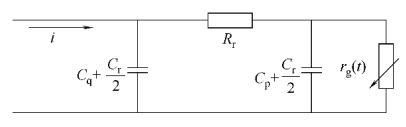
\includegraphics[width=\textwidth]{thesis_figure/anecdote_circuit}
		\caption{火花塞动态电路模型}
		\label{fig:hhscircuit}
	\end{minipage}
\end{figure}
其中$R_{r}$为火花塞内置电阻,其阻值可通过万用表测得或由生产商提供,通常为几千欧;$r_{g}$为火花塞气隙电阻,其阻值随火花塞的放电状态而发生变化,表征火花塞的非线性特性;
$C_{q}$、$C_{r}$、$C_{p}$分别表示前端中心电极、内置电阻、后端中心电极对火花塞金属外壳的寄生电容。火花塞内部可以看作静电场,因此火花塞动态模型可以如图\ref{fig:hhscircuit}所示。\
\subsection{火花塞间隙间的火花电阻}
图\ref{fig:hhscircuit}中的火花塞内置电阻$r_{g}$,前段中心电极对火花塞金属外壳的寄生电容$C_{q}$,内置电阻对火花塞金属外壳的寄生电容$C_{r}$,后端中心电极对火花塞
金属外壳的寄生电容$C_{p}$都可以通过有限元的方法进行计算\cite{zyl2011,wyj1999}。而火花塞间隙间的火花电阻$R_{g}$需要另外的方法进行计算。
\par 由Rompe-Weizel理论可知,火花电阻$r_{g}$是一个随时间变化的量,当火花间隙被击穿后,其随时间变化的关系为:
\begin{equation}
	\label{eqn:qxr}
	r_{g}=l_{g}(\frac{2\alpha}{p\int_{\infty}i_{g}^{2}dt})^{-0.5}
\end{equation}
式中,$l_{g}$为间隙宽度;$a$为火花系数;$p$为混合燃气压力;$i_{g}$为流过间隙的火花电流。
\par 间隙击穿后,火花电阻$r_{g}\leq5\Omega$,而火花塞电阻的阻值$5k\Omega\leq R_{r}\leq 20k\Omega$,所以$r_{g}\leq R_{r}$。考虑到高压点火导线的电阻$R_{w}$,火花
电流$i_{g}$主要有电容放电引起,根据电路理论可以得到:
\begin{align}
C &= C_{p}+\frac{C_{r}}{2}\\
\frac{du_{g}(t)}{dt}&=-\frac{1}{C}i_{g}(t)\\
\frac{di_{g}(t)}{dt}&=\frac{\alpha}{l_{g}^{2}p}u_{g}^{2}(t)i_{g}(t)-\frac{1}{C}\frac{i_{g}^{2}(t)}{u_{g}(t)}
\end{align}
设$t=t_{1}$时刻为电极产生电晕瞬间,$i_{g}(t_{1})=0$,$u_{g}(t_{1})=V_{br}$,$V_{br}$为火花塞气隙的击穿电压。利用数值算法,可以计算得到气隙电流$i_{g}(t)$及电压
$u_{g}(t)$。再代入式\ref{eqn:qxr}中即可求得$r_{g}$。
\subsection{离子电流检测电路等效电路模型}
根据火花塞的动态电路模型以及火花塞间隙间的火花电阻的计算公式,我们可以得到离子电流检测电路的等效电路模型如下:
\begin{figure}[!h]
	\centering
	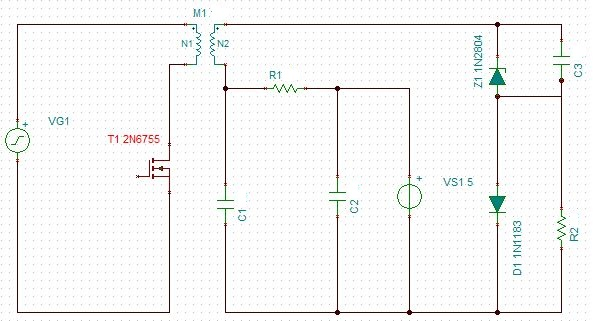
\includegraphics[width=0.8\textwidth]{thesis_figure/cmp_circuit}
	\caption{电路等效电路模型}
	\label{fig:cmp_circuit}
\end{figure}
\\其中$C_{1}=C_{q}+C_{r}/2$,$C_{2}=C_{p}+C_{r}/2$。由于火花塞间隙间的火花电阻$r_{g}$在不同时间的阻值不同,可以将该电路分为三种情况。
\subsubsection*{气隙断开的电路模型}
当MOSFET被点火控制信号触发后,在其导通时间内,一次线圈有电流通过,二次线圈出现感应电动势。但此时火花塞两极间的电压达不到击穿电压,此时火花塞气隙处于断开状态,此时在
MOSFET导通阶段有
\begin{gather}
	0\leq t\leq t_{1} \\
	r_{g}(t)=\infty \\                     
	i_{g}(t)=0
\end{gather}
时间$t_{1}$的计算即是计算火花塞气隙两段电压达到击穿电压$V_{br}$的时间。
\subsubsection*{气隙击穿瞬间的电路模型}
设火花塞气隙在$t=t_{1}$时开始产生电晕,$t=t_{2}$时被击穿,此过程火花塞由高阻抗特性变为低阻抗特性,即有
\begin{gather}
	t_{1}\leq t \leq t_{2}\\
	r_{g}=l_{g}(\frac{2\alpha}{p\int_{\infty}i_{g}^{2}dt})^{-0.5}
\end{gather}
\subsubsection*{气隙自持放电时的电路模型}
火花塞气隙击穿时出现电离现象,使得混合气被电离,从而形成了等离子通道,火花塞气隙进入自持放电阶段。此时火花塞两级电极间的电压维持稳定值
\cite{sincero2008arc,tseng1997experimentally},即有
\begin{gather}
	t_{2}\leq t \leq t_{3} \\
	u_{g}=U_{0}
\end{gather}
\section{小波分析}
\subsection{小波分析理论基础}
自从1822年傅里叶发表“热传导解析理论”以来,傅里叶变换一直是传统信号处理的基本方法。傅里叶变换能够满足大多数应用的需求,但是由于在进行
傅里叶变换的时候丢掉了时间信息,因此无法同时知道频域和时域情况下的信息。傅里叶变换在分析非平稳信号时表现出了严重的性能不足。然而实际中的信号
均包含大量的非平稳成分,比如突变、偏移等,然而这些非平稳信号往往反映了信号的重要特征。
\par 为了研究信号在局部时间段的频域特征,1946年Gabor提出了著名Gabor变换,之后发展成为了短时傅里叶变换(STFT),其基本思想是对信号加窗,然后对窗
内的信号进行傅里叶变换,因此它可以反映出信号的局部特性。但由于STFT的定义决定了其窗函数的大小和形状与时间和频率无关,因此对低频信号采用大时间窗进行
分析,而对于高频信号用小时间窗进行分析。小波变换继承了STFT的思想,它的窗口大小不变,但窗口形状可以改变,是一种时间窗和频率窗都可变的时频分析方法, 
即在低频部分具有较高的频率分辨率和较低的时间分辨率,在高频部分具有较高的时间分辨率和较低的频率分辨率,因此在时频都具有很强的表征信号局部特征的能力。
\par 在实际应用中,尤其是在计算机实现时,连续小波变换必须加以离散化,因此有必要讨论连续小波序列$\psi_{a,b}(t)$和连续小波变换$W_{f}(a,b)$的离散化。
在连续小波中,考虑小波函数
\begin{equation}
	\psi_{a,b}=|a|^{-\frac{1}{2}}\psi(\frac{t-b}{a})
\end{equation}
这里$b\in R$,$a\in R_{+}$,且$a\neq0$,$\phi$是容许的,为方便起见,在离散化中,总限制$a$只取正值,这样相容性条件就变为
\begin{equation}
	C_{\psi}=\int^{\infty}_{0}\frac{\mid \widehat{\psi}(\overline{\omega})\mid}{\mid \overline{\omega}\mid}d\overline{\omega} < \infty
\end{equation}
通常,把连续小波变换中尺度参数$a$和平移参数$b$的离散化公式分别取作$a=a_{0}^{j}$,$b=ka_{0}^{j}b_{0}$,这里$j\in Z$,扩展步长$a_{0}\neq 1$是固定值,
为方便起见,总是假定$a_{0}>1$(由于$m$可以取正也可以取负,因此这个假定无关紧要)。所以对应的离散小波变换函数$\psi_{j,k}(t)$即可写作
\begin{equation}
	\psi_{j,k}(t)=a^{-\frac{j}{2}}_{0}\psi(\frac{t-ka_{0}^{j}b0}{a_{0}^{j}})=a_{0}^{-\frac{j}{2}}\psi(a_{0}^{-\frac{j}{2}}t-kb_{0})
\end{equation}
而离散化小波系数则可表示为
\begin{equation}
	C_{j,k}=\int_{-\infty}^{\infty}f(t)\psi_{j,k}^{*}(t)dt=<f,\psi_{j,k}>
\end{equation}
其重构公式为
\begin{equation}
	f(t)=C\sum_{-\infty}^{\infty}\sum_{-\infty}^{\infty}C_{j,k}\psi_{j,k}(t)
\end{equation}
其中$C$是一个与信号无关的常数。由此可以看到信号序列$f(t)$可以由信号无关量$C$和小波函数$\psi$组成。
\subsection{多分辨率分析}
多分辨率分析是由一个尺度函数$\phi$建立起来的,因此多分辨率分析的建立等价于寻找尺度函数在多分辨率分析的框架下的性质。通过多分辨率分析可以从尺度函数$\phi$获得小波函数$\psi$,从而
可以对已知的信号进行分析和处理。
\par  Mallat在1989年给出了计算小波函数$\psi$的理论方法:
\par 设$(\{ V_{m};m\in Z\} ;\phi(t))$是一个正交多分辨率分析,则存在$\{ h_{k} \}\in l^{2}$使得下面的双尺度方程
\begin{equation}
	\phi(x) = \sum_{k}h_{k}\phi(2x-k)
\end{equation}
成立,并且利用尺度函数$\phi(x)$构造小波函数
\begin{equation}
	\psi(x)=\sum_{ki}g_{k}\phi(2x-k)
\end{equation}
其中$h_{k}=2\int_{-\infty}^{\infty}\phi(x)\overline{\phi(2x-k)}dx$,$g_{k}=(-1)^{k}\overline{h_{1-k}}$。
\par 根据上述理论多分辨率分析可以得到离散化的尺度函数和小波函数的获得方法。
\subsection{小波函数分析步骤}
第一步是采样。如果待分解的是模拟信号$f(t)$,选择$N=2^{n}$,得到采样信号值$a_{k}^{n}=f(\frac{k}{2^{n}})$,其中$k$的取值保证$\frac{k}{N}$位于信号$f(t)$发生的时间范围
之内,并在每个不小于$\frac{1}{N}$的时间段内都能取到采样信号$a_{k}^{n}=f(\frac{k}{2^{n}})$,于是可以用信号
\begin{gather}
f_{n}(x)=\sum_{k\in Z}a_{k}^{n}\phi(2^{n}x-k)
\end{gather}
对连续信号$f(t)$进行高精度的近似。
\par 第二步是分解。设信号$f_{n}(x)$逐级分解为
\begin{gather}
	f_{n}(x)=W_{n-1}(x)+W_{n-2}(x)+...+W_{l-1}(x)+f_{l-1}(x) \nonumber \\
			=W_{n-1}(x)+W_{n-2}(x)+...+W_{0}(x)+f_{0}(x)
\end{gather}
\par 其中
\begin{gather*}
W_{l-1}(x)=\sum_{k\in Z}b_{k}^{l-1}\psi(2^{l-1}x-k)\\
f_{l-1}(x)=\sum_{k\in Z}a_{k}^{l-1}\psi(2^{l-1}x-k)
\end{gather*}
系数$a_{k}^{l-1}$与$b_{k}^{l-1}$按照上标
从大到小的顺序从$l=n$开始直到$l=0$结束,满足
\begin{gather}
	b_{k}^{l-1}=\frac{a_{2k}^{l}-a_{2k+1}^{l}}{2}\\
	a_{k}^{l-1}=\frac{a_{2k}^{l}+a_{2k+1}^{l}}{2}
\end{gather}
\par 第三步是信号处理。将分解后的信号表示成下面的形式
\begin{gather}
	f_{n}(x)=\sum_{l=0}^{n-1}W_{l}(x)+f_{0}(x)\nonumber \\
			=\sum_{l=0}^{n-1}(\sum_{k\in Z}b_{k}^{l}\psi(2^{l}x-k))+\sum_{k\in Z}a_{k}^{0}\phi(x-k)
\end{gather}
信号处理的过程就是根据实际情况对$b_{k}^{l}$作适当的修正。例如信号处理的目的是去噪,那么可以将不可能存在的频率范围对应的系数$b_{k}^{l}$设置为0;如果信号处理用于压缩,则可以根据压缩比的
大小及小波系数的取值范围设置适当的阈值,当小波系数绝对值小于阈值时,设置$b_{k}^{l}$为零。
\par 第四步是信号重构。设重构后的信号值满足
\begin{equation}
	\widetilde{f_{n}}(x)=\sum_{k\in Z}a_{k}^{n}\phi(2^{n}x-k)
\end{equation}
则上述信号值可以通过下面的递推过程得到
\begin{equation}
	\widetilde{a}^{l}=\widetilde{L}U\widetilde{a}^{l-1}+\widetilde{H}U\widetilde{b}^{l-1}, l=1,2,3,...,n
\end{equation}
其中$\widetilde{a}^{l}$和$\widetilde{b}^{l}$,$l=0,1,2,3,...,n$是根据第二、第三步得到的修正系数。
\subsection{小波分析的特点}
\begin{enumerate}[1)]
	\item \textbf{灵活性}\quad 由于小波基函数$\phi(x)$不是唯一的,只需要满足构造小波函数的条件即可,因而就有许多构造小波的方法。不同的小波函数有不同的特性,可以用来逼近不同的信号
以便得到最佳结果。而傅里叶变换只用正弦信号逼近任意信号,没有选择的余地,逼近效果不能理想化。
	\item \textbf{快速性}\quad 由于有了多分辨率分析,可以提高小波分析的效率。通过尺度函数和两尺度关系推导小波系数,在未知小波函数的解析表达式情况下也可以得到分析的结果。并且在频带细分下可以起到显微镜的作用,
这是傅里叶分析无法比拟的。
	\item \textbf{双域性}\quad 小波分析是时频分析,可以时域和频域同时揭示信号的特征。而傅里叶变换只能在单域中显示信号特性。
	\item \textbf{深刻性}\quad 小波理论是建立实变函数、复变函数、泛函分析、调和分析等近代数学理论基础上的,具有深刻的理论基础。
\end{enumerate}
\subsection{常见的可离散小波}
\par  db小波的全称是Daubechies小波。Daubechies小波是由世界著明的小波分析学者Ingrid Daubechies构造的小波函数,我们一般简写成dbN,N是小波的阶数。小波函数$\psi(t)$和
尺度函数$\phi(t)$中的支撑区为2N-1,$\psi(t)$的消失矩为N。dbN小波具有较好的正则性,即该小波作为稀疏基所引入的光滑误差不容易被察觉,使得信号重构过程比较光滑。dbN小波的特点是随着阶次(序列N)的增大消失矩阶数越大,其
中消失矩越高光滑性就越好,频域的局部化能力就越强,频带的划分效果越好,但是会使时域紧支撑性减弱,同时计算量大大增加,实时性变差。另外,除N=1外,dbN小波不具有对称性(即非线性相位),即在对信
号进行分析和重构时会产生一定的相位失真。dbN没有明确的表达式(除了N=1外,N=1时即为Haar小波)。
\par  symlet小波函数是Ingrid Daubechies提出的近似对称的小波函数,它是对db函数的一种改进。Symlet小波系通常表示为symN (N=2,3,…,8)。symN小波的支撑范围为2N-1,消失矩为N,同时也具备较好的正则性。该小波与dbN小波相
比,在连续性、支集长度、滤波器长度等方面与dbN小波一致,但symN小波具有更好的对称性,即一定程度上能够减少对信号进行分析和重构时的相位失真。
\par  coiflet小波是根据R.Coifman的要求,由Daubechies构造的,它具有coifN (N=1,2,3,4,5)这一系列。Coiflet的小波函数$\psi(t)$的2N阶矩为零,尺度函数$\phi(t)$的2N-1阶矩为零。$\psi(t)$和$\phi(t)$的支撑长度为6N-1。
Coiflet的$\psi(t)$和$\phi(t)$具有比dbN更好的对称性。
\par  dmey小波全称是discrete meyer小波,也就是离散meyer小波。meyer小波由法国数学家Yves Meyer于1990年提出。
\subsection{离散小波之间的比较}
在不同的应用领域,小波基的选取标准不同,一般的选择原则如下:
\par (1)正交性。正交性源于数学分析的简单和工程应用中便于理解操作,表现为小波基的可微性。
\par (2)紧支性。紧支集保证有优良的时频局部特性,也利于算法的实现。若小波函数$\psi(t)$有紧支集,则称小波基函数是紧支的。紧支集小波满足空间局部性的要求,特别在为了得到有限长度的滤波器组$h(n)$,$g(n)$
;避免滤波过程中的截断误差,要求小波基为紧支的。
\par (3)对称性。对称小波基具有线性相位特性,对图像边缘作对称边界扩展时,重构图像边缘部分失真较小,有利于复杂特性的分析。对称和反对称的尺度函数和小波函数是非常重要的,因为可以构造紧支的正则小波基,而且
具有线性相位。Daubechies已经证明,除了Haar小波基,不存在对称的紧支正交小波基。而对于双正交小波基,可以合成具有对称或反对称的紧支小波基。
\par (4)正则性。正则性是函数光滑程度的一种描述,函数频域能量的一种度量。正则性越高,小波分析效果越好。
\par (5)消失矩问题。为了提高衰减程度,要求所用的基函数具有一定的消失矩。消失矩的阶数越大,精细尺度下高频部分数据值就越有可能存在许多小至可以忽略的点。
下表\ref{tab:lsxb}所示的是所有的可以进行离散小波变换的小波比较\cite{wxf2003}。
\begin{table}[!h]
	\centering
	\caption{可离散变换的小波函数比较}
	\label{tab:lsxb}
	\begin{tabular}{c|c|c|c|c}
	\toprule[1.5pt]
	小波名称&正交性&双正交性&紧支撑性&支撑长度\\
	\midrule[1pt]
	db&是&是&是&2N-1\\
	sym&是&是&是&2N-1\\
	dmey&是&是&是&有限长度\\
	coif&是&是&是&6N-1\\
	\midrule[1pt]
	\multicolumn{5}{c}{}
	\end{tabular}
	\begin{tabular}{c|c|c|c|c}
	\midrule[1pt]
	小波名称&滤波器长度&对称性&小波函数消失矩阶数&尺度函数消失矩阵数\\
	\midrule[1pt]
	db&2N&对称&N&-\\
	sym&2N&近似对称&N&-\\
	dmey&[-8,8]&对称&-&-\\
	coif&6N&近似对称&2N&2N-1\\
	\bottomrule[1.5pt]
	\end{tabular}
\end{table}
基本小波类型的选择较难总结成一般原则,只能针对具体问题提出具体原则。\par
例如对于分段多项式结构组成的信号,db小波比较适用;如果信号含正弦分量或高频振荡,则局部三角函数基比较合适。如何
根据分析信号的特点,结合任务来优化设计小波函数一直是值得探讨的问题,迄今为止还没有系统完整的总结。且对于一些特定的离散问题,还可以通过利用多分辨率分析的方法自己构造离散的尺度函数和
小波函数。
\section{高斯曲线拟合}
\subsection{高斯函数}
高斯函数的应用范围很广,在自然科学、社会科学、数学以及工程学等领域都能看到它的身影。高斯函数的形式为:
\begin{equation}
	f(x)=ae^{-\frac{(x-b)^2}{c^2}}
\end{equation}
其中$a$,$b$,$c$为实常数,且$a>0$。
\par  $c^2=2$的高斯函数是傅里叶变换的特征函数。这就意味着高斯函数的傅里叶变换不仅仅是另一个高斯函数,而且是进行傅里叶变换的函数的标量倍。
高斯函数的不定积分是误差函数。\par
在自然科学、社会科学、数学以及工程学等领域都有高斯函数的身影,比如在统计学与机率论中,高斯函数是正态分布的密度函数,根据中心极限定理,他是复杂
总和的有限几率分布。
\subsection{离子电流拟合原理和方法}
Saitzkoff\cite{saitzkoff1996ionization}在缸内气体完全燃烧并且达到热化学平衡情况下推导了火焰后期的离子电流的理论公式。
\begin{equation}
	\frac{I}{I_{m}}=\frac{1}{\frac{p}{p_m}}^{\frac{1}{2}-\frac{3}{4}\frac{\gamma -1}{\gamma}}e^{-\frac{E_i}{2\kappa T_m}[\frac{1}{(\frac{p}{p_m})^{\frac{\gamma -1}{\gamma}}}-1]}
\end{equation}
其中各物理量含义如表\ref{tab:gswllhy}所示。
\begin{table}[htb]
	\centering
	\caption{\label{tab:gswllhy}公式物理量含义}
	\begin{tabular}{cc}
		\toprule[1.5pt]
		物理量&含义\\
		\midrule[1pt]
		I&离子电流\\
		$I_m$&离子电流最大值\\
		p&缸压\\
		$p_m$&缸压最大值\\
		$T_m$&最大温度\\
		$\gamma$&热力学系数\\
		$\kappa$&波尔兹曼常数\\
		$E_i$&离子电流能量\\
		\bottomrule[1.5pt]
	\end{tabular}
\end{table}
该公式与高斯函数相近。所以可以将火焰后期的离子电流近似拟合成高斯曲线。\par
L.Eriksson和L.Nielsen\cite{eriksson1996ignition,eriksson1997closed,eriksson1997ionization}采用该方法能够准确地估计缸压最值对应相位,从而可以
自适应调整点火提前角,提高了发动机的燃烧效率。Magnus Hellring等人也通过了拟合曲线的方法控制了缸压峰值相位的位置\cite{hellring2001comparison}。\par
而由于排气过程不能将缸内的所有废弃排除缸内,断油循环和断火循环中仍然存在部分带NO离子
的废弃,仍然可以检测到离子电流。同样道理,在正常循环的点火之前由于存在部分废气,离子电流检测电路可以检测到轻微的离子电流信号。这部分废弃导致的离子电流信号也可以用高斯函数近似分析。
由此整个检测到的离子电流信号可以用两个高斯曲线拟合来进行分析。





